\documentclass[english,inz,shortabstract]{iithesis}

\usepackage[utf8]{inputenc}
\usepackage{natbib}
\usepackage[nottoc,notlot,notlof]{tocbibind}
\usepackage{graphicx}
\usepackage{enumitem}
\usepackage{hyperref}
\usepackage[justification=centering]{caption}
\usepackage{lipsum}
\usepackage{listings}
\usepackage{color}
\usepackage{todonotes}
\usepackage{dirtree}
\usepackage{float}

\definecolor{codegreen}{rgb}{0,0.6,0}
\definecolor{codegray}{rgb}{0.5,0.5,0.5}
\definecolor{backcolor}{rgb}{0.90,0.90,0.90}
\definecolor{codered}{RGB}{216, 38, 81}
\definecolor{darkblue}{rgb}{0.0,0.0,0.6}

\lstdefinestyle{mystyle}{
	backgroundcolor=\color{backcolor},
	commentstyle=\color{codegreen},
	keywordstyle=\color{codered},
	numberstyle=\tiny\color{codegray},
	basicstyle=\ttfamily\scriptsize,
	breakatwhitespace=false,
	breaklines=true,
	captionpos=b,
	keepspaces=true,
	numbers=none,
	numbersep=5pt,
	frame=single,
	showstringspaces=false
}

\lstdefinelanguage{XML}
{
  morestring=[b]",
  morestring=[s]{>}{<},
  morecomment=[s]{<?}{?>},
  identifierstyle=\color{darkblue},
  morekeywords={name,filename}
}

\lstdefinelanguage{rubiC}
{
	language = C,
	morekeywords = {int32_t, bool_t}
}

\lstdefinelanguage{mybash}
{
	language = bash,
	morekeywords = {mkdir, catkin, rosdep, apt, roslaunch, rostopic, rosservice},
	deletekeywords = {command, false}
}

\lstset{
	style=mystyle,
	literate={~} {$\sim$}{1},
	columns=fullflexible,
	aboveskip=0.6\baselineskip,
	belowskip=0.0pt
}

\newcommand{\filedesc}[1] {
\dotfill
% \fbox{
\vspace{0.1cm}
\begin{minipage}[t]{6cm}
	#1
\end{minipage}
\vspace{0.1cm}
% }
}

\newcommand{\val}[1]{\textbf{\textsf{#1}}}

\setlength{\DTbaselineskip}{\baselineskip}

\newcommand{\oldrovername}{$\aleph_1$\ }
\newcommand{\rovername}{$\aleph_2$\ }

\newcommand{\todomma}[1]{\todo[author=mma]{#1}}

\englishtitle   {Control software and simulation environment \fmlinebreak for the Aleph2 robot -- a Mars rover prototype}
\polishtitle    {Oprogramowanie do kontroli i symulacji \fmlinebreak robota Aleph2 -- prototypu łazika marsjańskiego}
\author         {Błażej Sowa}
\advisor        {dr Marek Materzok}
%\date          {}

\englishabstract{
	The \oldrovername (pron. aleph one) robot is a Mars rover prototype being developed since 2015 by the student research group \textit{Continuum}, operating at the University of Wroclaw. One of the team's most outstanding achievements is 2nd place at the \textit{University Rover Challenge 2017}, where the rover proved itself well performing tasks in the desert in Utah.\\
	The thesis focuses on the implementation of the hardware abstraction layer and the simulation environment created for the successor of the aforementioned robot, \rovername (pron. aleph two). The software is largely based on the use of the Robot Operating System (ROS), ros\_control framework and Gazebo simulator.
}

\polishabstract{
	Robot \oldrovername (czyt. alef jeden) to prototyp łazika marsjańskiego rozwijany od 2015 roku przez koło naukowe \textit{Continuum}, działające na Uniwersytecie Wrocławskim. Do jednych z najwybitniejszych osiągnięć drużyny można zaliczyć 2. miejsce na zawodach \textit{University Rover Challenge 2017}, gdzie łazik bardzo dobrze sprawdził się wykonując zadania na pustyni w Utah.\\    
	Praca skupia się na implementacji warstwy abstrakcji sprzętowej oraz środowisku symulacyjnym stworzonych na potrzeby następcy wyżej wspomnianego robota, \rovername (czyt. alef dwa). Oprogramowanie opiera się w znacznym stopniu na wykorzystaniu Robot Operating System (ROS), frameworku ros\_control i symulatora Gazebo. 
}

\begin{document}

\chapter{Introduction}

\section{Background}
The NASA's \textit{Mars Exploration Rover} mission has inspired various annual robotic competitions for university level students. The challenge is to build a robot that would help early explorers on Mars. 
The \textit{Rover Challenge Series} is a series of such competitions run by the \textit{Mars Society}. Among the most popular are \textit{University Rover Challenge} (hosted since 2007) and \textit{European Rover Challenge} (hosted since 2014).

The tasks on the competitions often include:
\begin{itemize}[itemsep=0pt, parsep=2pt, topsep=0pt]
	\item Navigating through rough terrain
	\item Picking up and transporting objects
	\item Flipping switches on the control panel 
	\item Collecting and examining soil samples
\end{itemize}

\textit{Continuum} (also known as \textit{Team Continuum} or \textit{Continuum Rover Team}) is a student research club from University of Wroclaw whose main focus is to build and improve its Mars rover prototype and compete in the challenges. The team has operated since 2014 and debuted with the \oldrovername (pron. aleph one) robot, scoring 3rd place at \textit{University Rover Challenge 2016} and 2nd place at \textit{University Rover Challenge 2017}.

Now, the team is focused on improving the \rovername rover (Fig. \ref{fig:lazik1} and \ref{fig:lazik2}), which is the next iteration of the \oldrovername robot. 


\begin{figure}[ht]
	\hspace*{\fill}
	\begin{minipage}{.45\textwidth}
	  \centering
	  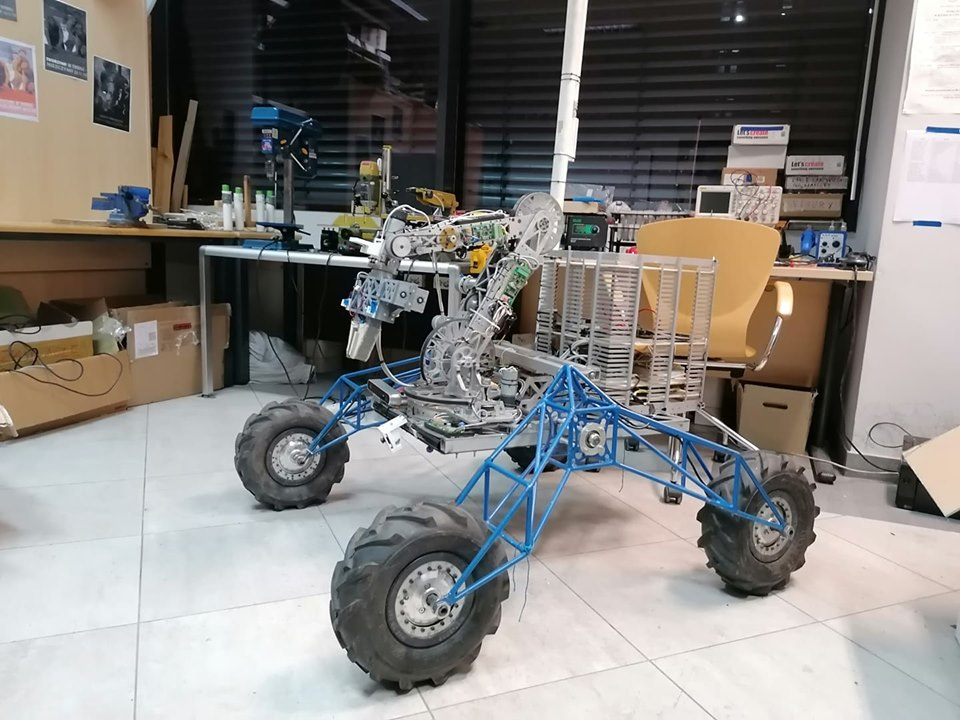
\includegraphics[height=4cm]{img/lazik1.jpg}
	  \caption{The current appearance of the \rovername rover}
	  \label{fig:lazik1}
	\end{minipage}
	\hfill
	\begin{minipage}{.45\textwidth}
	  \centering
	  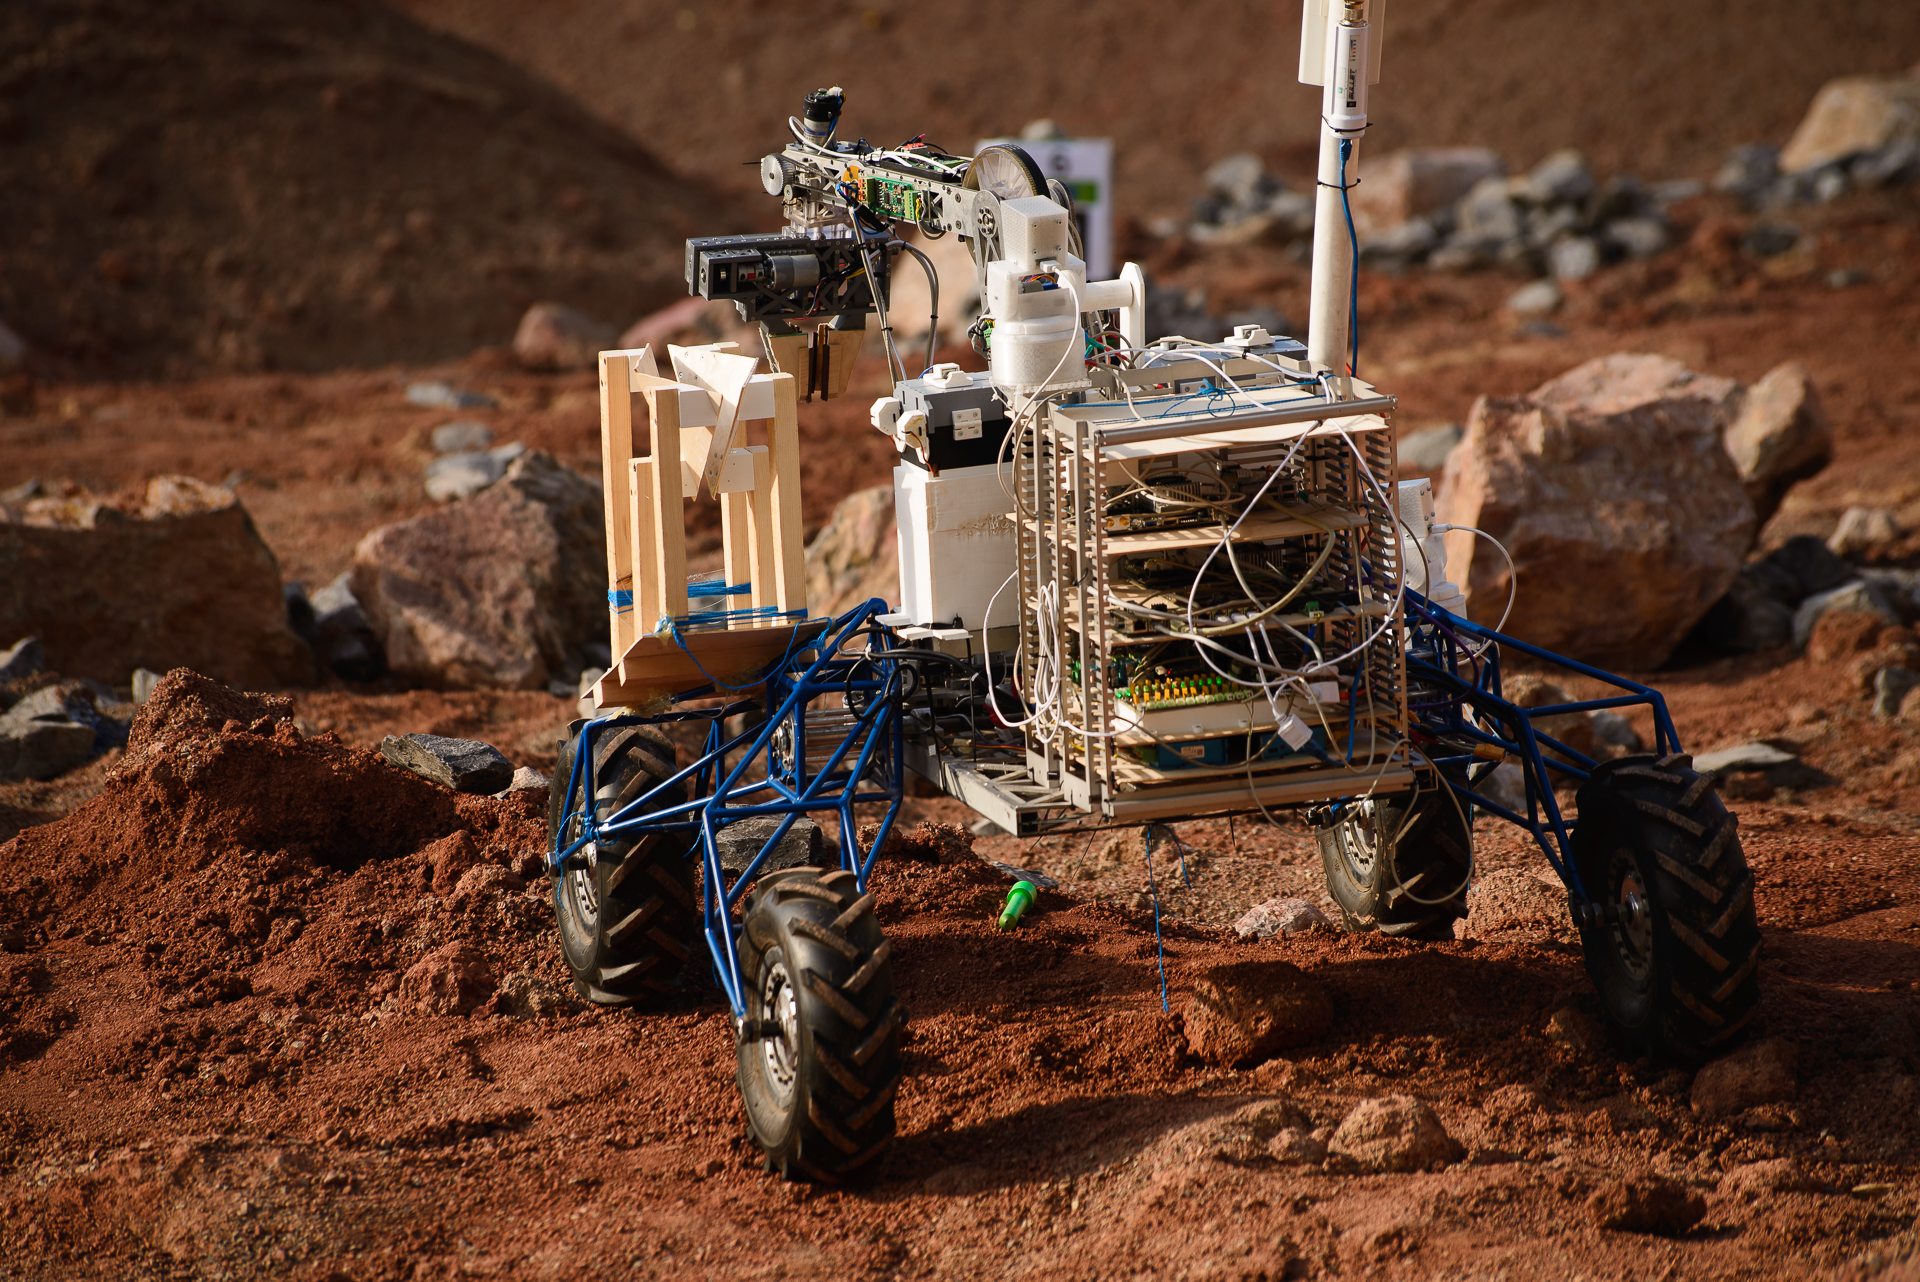
\includegraphics[height=4cm]{img/lazik2.jpg}
	  \caption{\rovername performing a task at the \textit{European Rover Challenge 2019}}
	  \label{fig:lazik2}
	\end{minipage}
	\hspace*{\fill}
\end{figure}

\section{Motivation}
Although the \oldrovername rover is a well-proven construction piece, its software responsible for robot control and communication with the hardware leaves a lot of room for improvement. The main problems identified are:
\begin{itemize}
	\item \textbf{Unstable implementation} -- the software responsible for the drivetrain often fails to communicate with the motor drivers due to  partial implementation of the communication protocol and various race conditions.
	\item \textbf{Hard-coded configuration} -- all of the configuration (e.g. IDs of the motor drivers, joint names and limits) is embedded into the source code. This makes it needlessly difficult to reconfigure the programs after making changes to other robot subsystems (hardware or software).
	\item \textbf{Lack of abstraction layers} -- the software does not provide any libraries for the implemented controllers or communication protocols. All of these components are placed into single executables. This makes it hard to reuse the code for other purposes.
\end{itemize}
These issues, combined with the passion for robots, were the main reasons that led to the decision of making new control software for the \rovername rover.

\section{Goals} \label{goals}
To address the aforementioned issues with the previous system, a set of design assumptions that the new software has to meet has been defined. The main assumptions include:

\begin{itemize}
	\item \textbf{Extensive use of open source software} -- by relying on widely used and well tested open source projects, the software can become more stable and be developed faster.
	\item \textbf{No hard-coded configuration} -- the programs should not assume much about the hardware they are running on. Instead, they should read the configuration at runtime. The configuration should be well-documented and easily editable.
	\item \textbf{Hardware abstraction layer} -- the software should deliver an abstraction over the hardware it is communicating with by providing interfaces that define its capabilities. This should greatly improve the reusability of the code. 
	\item \textbf{Simulation environment} -- the software should provide the ability to simulate the robot operation in a virtual world. The simulation should be able to run the same set of controllers (ideally, with the same configuration) and provide the same control interfaces as the real robot.
\end{itemize}


\section{Used technologies}
This section describes some of the main concepts of technologies the software is based on, which are essential in order to understand certain parts of this thesis.

	\subsection{ROS}
	\begin{quote}
		The Robot Operating System (ROS) is a flexible framework for writing robot software. It is a collection of tools, libraries, and conventions that aim to simplify the task of creating complex and robust robot behavior across a wide variety of robotic platforms.
		\cite{ros:about}
	\end{quote}

	This is a brief overview of the concepts related to ROS. A more in-depth information, as well as tutorials, can be found in the documentation \cite{ros:documentation} and in books, such as \cite{ros:mastering}.

	ROS was founded in 2007 by Willow Garage, a robotics research lab and technology incubator devoted to developing hardware and open source software for personal robotics applications \cite{ros:willowgarage}. In 2013, the project was taken over by the Open Source Robotics Foundation (OSRF), a non-profit organization founded by members of the global robotics community.

	It is important to note that ROS in itself is not a real operating system (in the sense of process management) but rather a meta-operating system that runs on top of Unix-based platforms. It provides a layer for communication and management of processes running in a heterogeneous computer cluster (hence the term meta-operating system).

	The basic concepts of ROS include:
	\begin{description}[style=nextline]
		\item [Computation graph] \hfill
		Peer-to-peer network of ROS nodes that are running in a computer cluster.
		\item [Nodes] 
		Processes that perform computation. They can communicate with each other via topics, services or Parameter Server. A typical robot control system will consist of many nodes. For example, one for communication with the hardware, one that performs path planning, one that provides graphical interface, and so on.
		\item [Topics] 
		Named buses over which nodes exchange messages. Nodes do not assume the recipient of the messages they send. Instead, they \textit{publish} to the specified topic. The nodes that want to receive these messages can \textit{subscribe} to the same topic. There is no limit on publishers and subscribers, but only one message type can be sent to one topic.
		\item [Services] 
		Services are similar to topics, but instead of asynchronous stream of data, they allow for synchronous request / reply interactions. They allow one node to call a function that executes in another node and get the result. Two nodes cannot provide the service with the same name.
		\item [Message types]
		For two nodes to successfully communicate via topics or services, a message type definition has to be shared between them. Message types are defined by a simplified description format where a set of fields is listed. Each field contains a name and a type (either a built-in type, an array or another message). Service types use the same description format but both request and reply types are defined.
		\item [Master]
		A program that is essential to run the computation graph. It enables individual nodes to locate each other; keeps track of the running nodes, registered publishers, subscribers, services. The master also provides the Parameter Server.  
		\item [Parameters]
		Globally viewable data entries stored in the Parameter Server that can be retrieved by nodes at runtime. Their primary use is to store static, non-binary data such as configuration for the starting nodes.
		\item [Launch files]
		Describe a set of nodes to run together and parameters to load on the Parameter Server. They provide an easy way to start the whole subsystem by executing only one command. 
		\item [URDF model]
		Unified Robot Description Format (URDF) allows to represent the robot model in a human-readable format, which can be useful in the ROS ecosystem. The elements of the robot, together with their collision, inertial and physical properties, are described by \textit{links}. The connections between \textit{links} (parent and child) are specified by \textit{joints}. (see Fig. \ref{fig:husky}) 
		\item [Packages]
		Main unit for organizing software in ROS. A single package may contain nodes, libraries, message and service type definitions, launch files, URDF models, configuration files and other pieces of software that constitute a useful module. A package also typically defines its dependencies as either other ROS packages or ROS-independent tools, libraries.

	\end{description}

	\begin{figure}[ht]
		\centering
		\captionsetup{margin=2cm}
		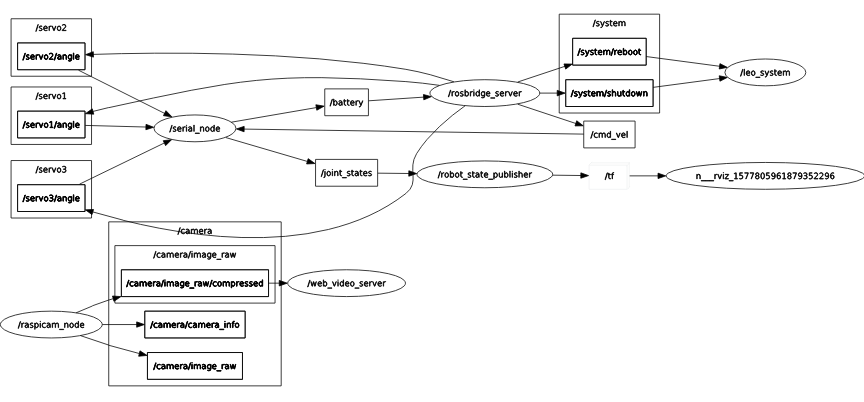
\includegraphics[width=\textwidth]{img/rqt_graph.png}
		\caption{An example visualization of ROS computation graph, created with  \href{http://wiki.ros.org/rqt_graph}{rqt\_graph} tool.}
		\label{fig:ros_graph}
	\end{figure}

	\begin{figure}[ht]
		\centering
		\captionsetup{margin=1cm}
		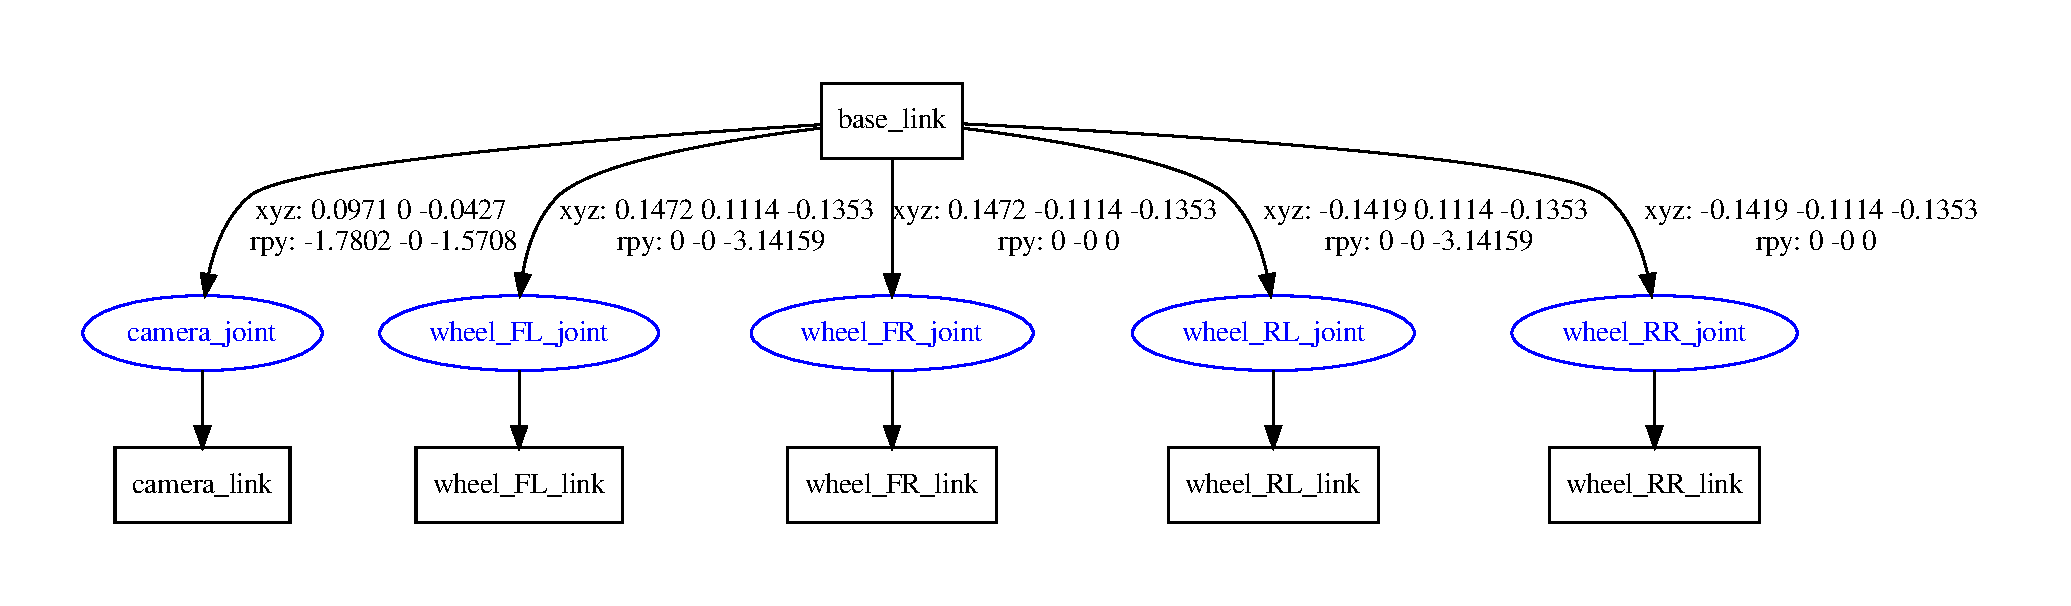
\includegraphics[width=\textwidth]{img/leo_description.pdf}
		\caption{An example visualization of URDF model of four-wheeled robot with a camera, created with \href{http://wiki.ros.org/urdf\#Visualization}{urdf\_to\_graphviz} tool. Black rectangles represent links and blue ovals represent joints.}
		\label{fig:husky}
	\end{figure}

\pagebreak

		\subsubsection{Built-in tools}
		Apart from the communication libraries, the core ROS packages provide many useful utilities, such as command line tools:

		\begin{itemize}[itemsep=0pt, parsep=2pt, topsep=0pt]
			\item \textbf{roscore} -- starts ROS Master, Parameter Server and \textsf{rosout} \cite{ros:rosout} logging node,
			\item \textbf{rosrun} -- runs a node located in an arbitrary package,
			\item \textbf{roslaunch} - launches a set of nodes specified in a launch file, starts roscore if it is not running already,
			\item \textbf{rosnode} -- lists and prints information about running nodes, pings or kills a specified node,
			\item \textbf{rostopic} -- lists and prints information about active topics, displays messages published on a specified topic or publishes on one by itself,
			\item \textbf{rosservice} -- lists and prints information about the advertised services, calls a service and displays the response,
			\item \textbf{rosdep} -- downloads and installs the dependencies of a given package.
		\end{itemize}
		They also provide graphical tools:

		\begin{itemize}[itemsep=0pt, parsep=2pt, topsep=0pt]
			\item \textbf{RQt} -- a framework for GUI applications in ROS. It enables development of Qt-based widgets that can communicate with other nodes running in the system. The base plugins provide many useful functions, such as publishing messages, displaying log messages, plotting data published on topics, visualizing the computation graph and many others (see Fig. \ref{fig:rqt}),
			\item \textbf{RViz} -- a 3D visualization tool for ROS. It provides plugins for displaying various things that the robot perceives, such as current state of the joints, camera images, data from the sensors, computed localization, occupancy map and many more. It can also be used to interact with the robot via, for example, navigation goal publishing or motion planning execution (see Fig. \ref{fig:rviz_pr2}).
		\end{itemize}

		\begin{figure}[ht]
			\centering
			\captionsetup{margin=2cm}
			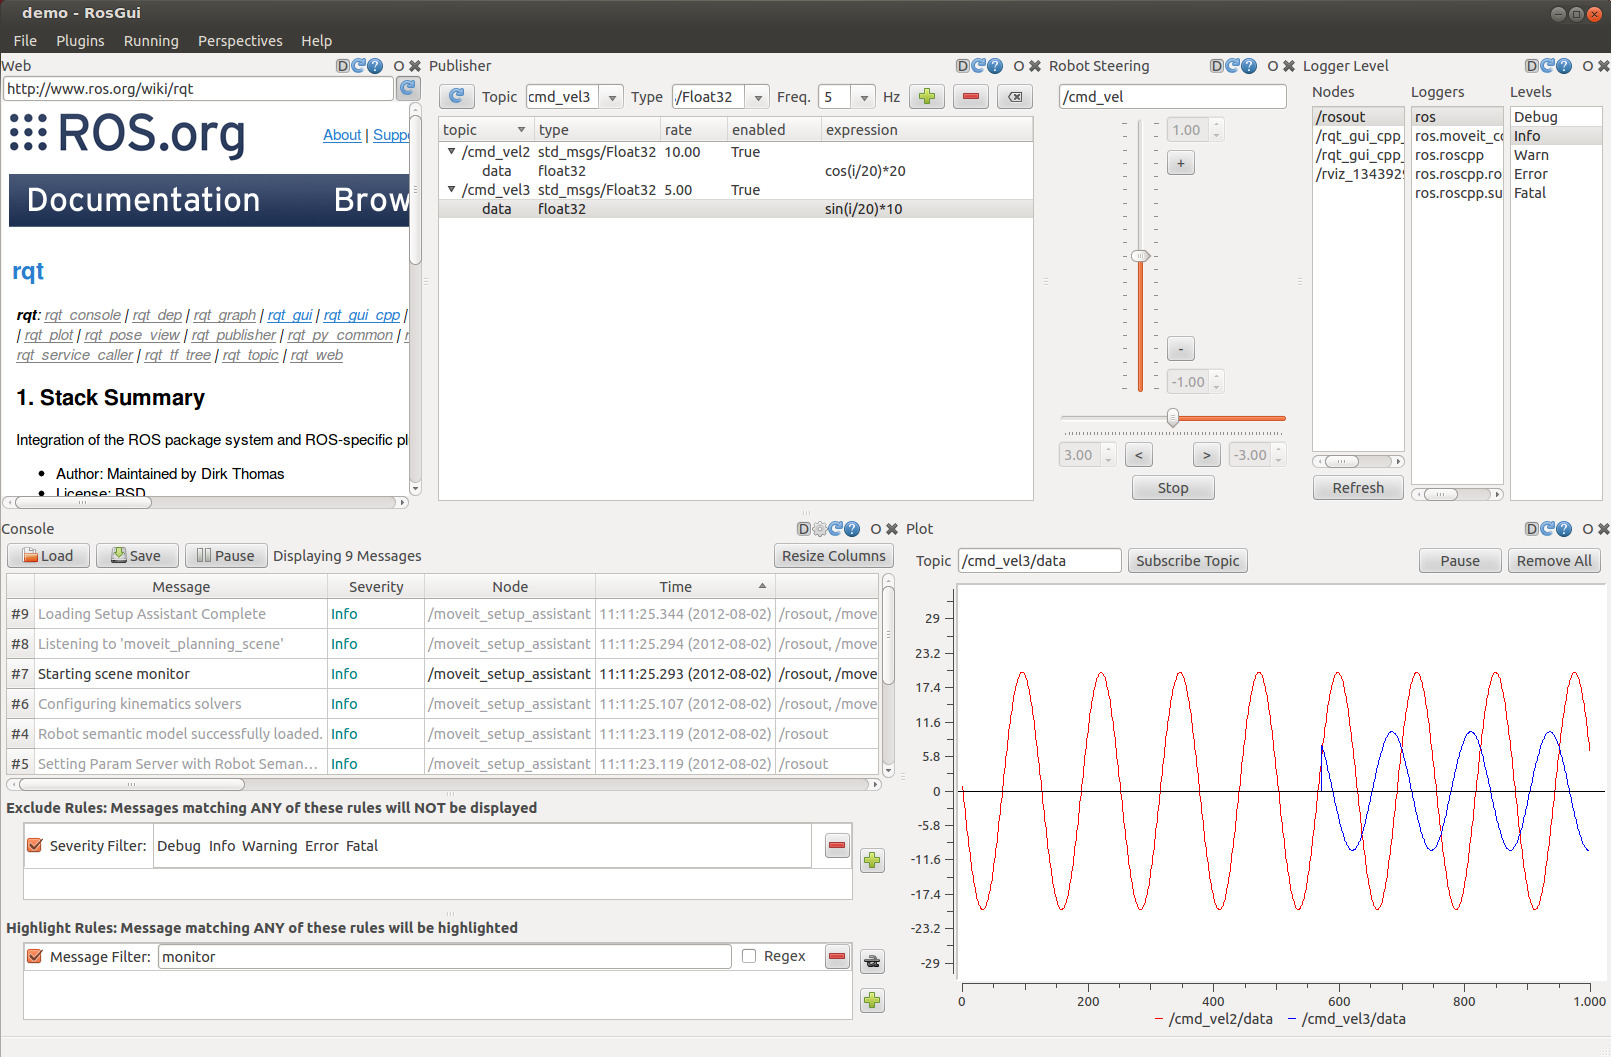
\includegraphics[height=6cm]{img/rqt.png}
			\caption{An example screenshot of RQt (Source: \cite{ros:rqt})}
			\label{fig:rqt}
		\end{figure}

\pagebreak

		\begin{figure}[ht]
			\centering
			\captionsetup{margin=2cm}
			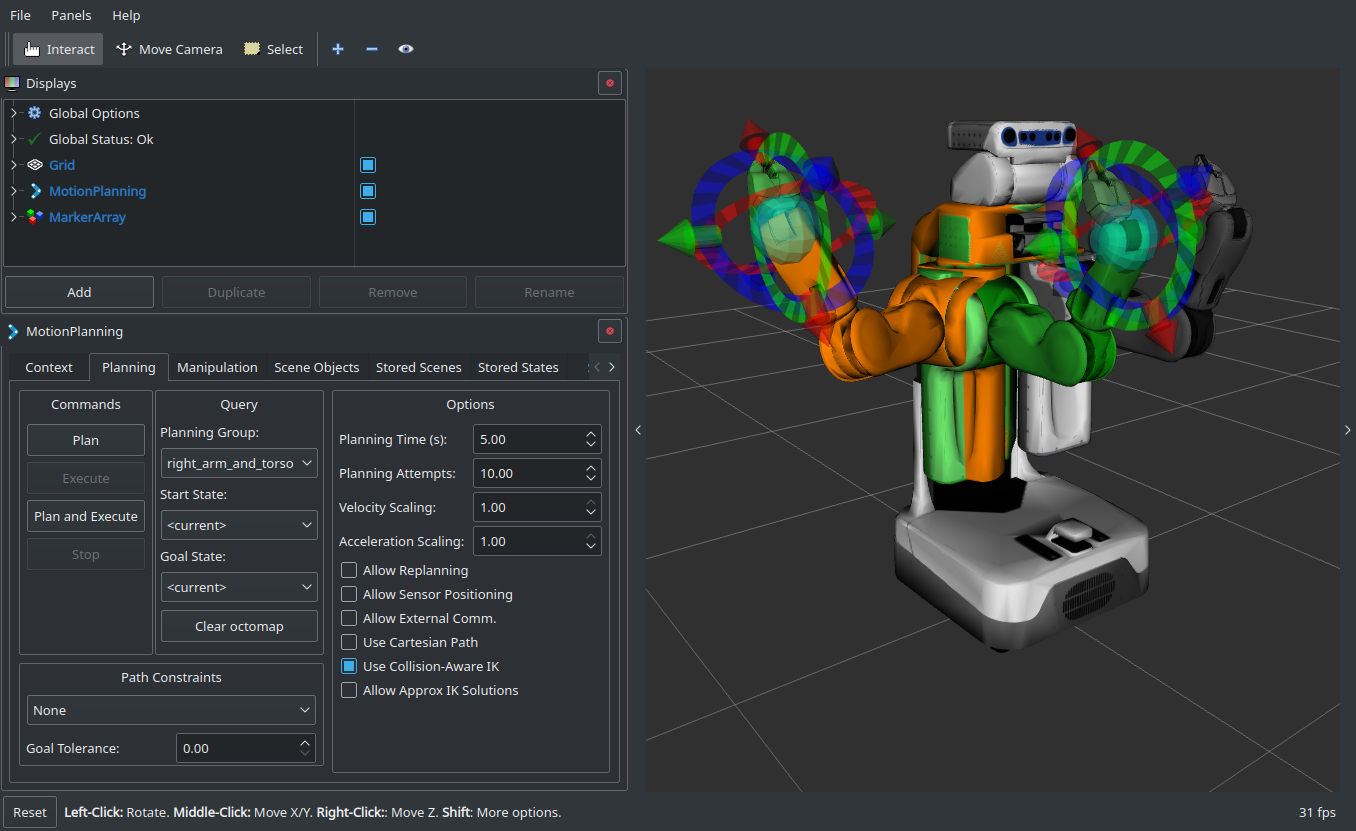
\includegraphics[height=6cm]{img/rviz_pr2.png}
			\caption{RViz utilizing motion planning plugin to move the joints on the PR2 robot}
			\label{fig:rviz_pr2}
		\end{figure}

	\subsection{ros\_control}
	
	\begin{quote}
		The ros\_control framework provides the capability to implement and manage robot controllers with a focus on both real-time performance and sharing of controllers in a robot-agnostic way.
		\cite{ros_control:paper}
	\end{quote}

	\textsf{ros\_control} (also referred as \textsf{ROS control}) was developed as a hardware independent version of \textsf{pr2\_controller\_manager}, which is a framework specific to the PR2 robot. Its core functionality can be summarized by the following components:

	\begin{description}[style=nextline]
		\item [Hardware interfaces]
		Provide a standardized way for communication between controllers and the hardware abstraction layer by sharing resources across them. The most common hardware interfaces include: state interface (for getting the current joint state) and command interfaces (for sending command to the joints, such as effort, velocity or position commands).   
		\item [RobotHW]
		A base class for abstracting custom robot hardware. It provides functions to register and manage hardware interfaces and performs resource conflict checking. To implement a hardware abstraction layer for a robot, the user has to write a derived class that looks similar to this:
		\lstinputlisting[language=C++]{lst/robot_hw.lst}
		\item [Controllers]
		Communicate with the hardware abstraction layer by accessing resources that are shared through hardware interfaces. Some example controller types available in \textsf{ros\_control} include:
			\begin{itemize}
				\item \textsf{joint\_state\_controller/JointStateController} - reads joint states and publishes them on a ROS topic; requires state interface,
				\item \textsf{velocity\_controllers/JointVelocityController} - listens for velocity commands and forwards them to the hardware abstraction layer; requires velocity interface
				\item \textsf{effort\_controllers/JointPositionController} - listens for position commands and forwards effort commands to the hardware abstraction layer; uses a closed-loop controller to get to joint to the specified position; requires effort and state interfaces
			\end{itemize}
		\item [Controller Manager]
		Is responsible for managing the life cycle of the controllers. Provides its functionality through ROS services. It allows to list, load, unload, start or stop controllers. 
		\begin{figure}[ht]
			\centering
			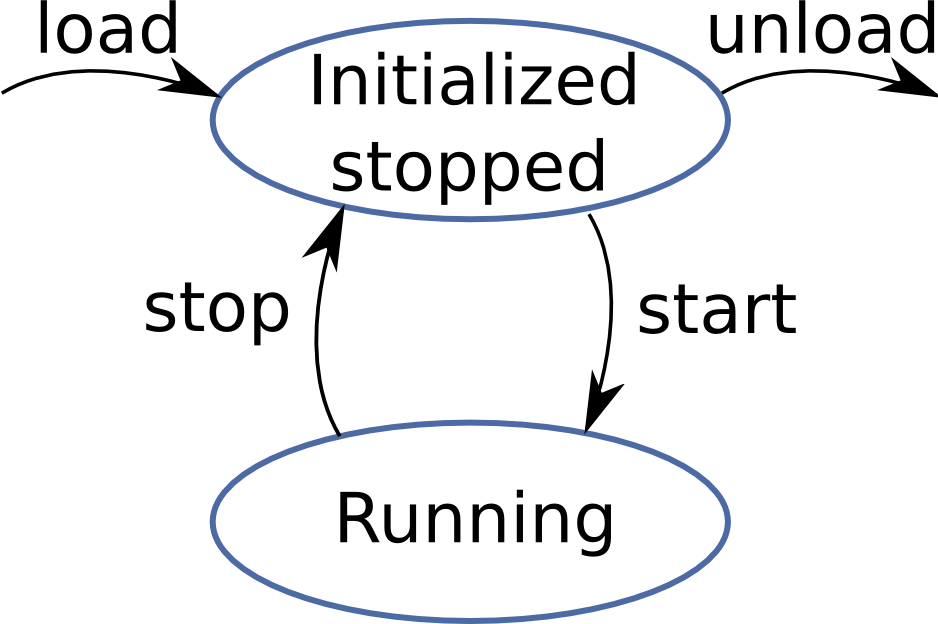
\includegraphics[height=3cm]{img/controller_life.png}
			\caption{Life cycle of a controller (Source: \cite{ros_control:cm_wiki})}
			\label{fig:controller_life}
		\end{figure}

	\end{description}

% \pagebreak
	
	\begin{figure}[ht]
		\centering
		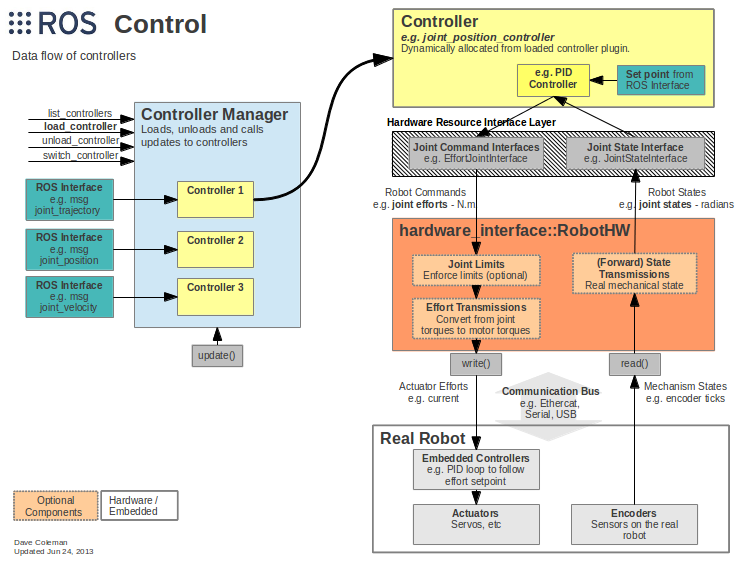
\includegraphics[width=\textwidth]{img/ros_control.png}
		\caption{ROS control overview (Source: \cite{ros_control:wiki})}
		\label{fig:ros_control}
	\end{figure}

	\subsubsection{Control loop}
	After writing the hardware abstraction layer for the robot, the user has to implement a control loop that utilizes the Controller Manager, in order to be able to load some controllers. A sample control loop may look similar to this:

	\lstinputlisting[language=C++]{lst/control_loop.lst}

\pagebreak

	\subsection{Gazebo}
	Gazebo provides an open-source 3D simulation environment, mainly for simulating robots. It incorporates high-performance physics engines, such as Open Dynamics Engine (ODE), Bullet, Dynamic Animation and Robotics Toolkit (DART), etc. and supplies a realistic rendering of the environment. It can model robot behavior, as well as, various sensors, such as cameras, laser range finders, IMU, GPS.

	Gazebo uses its own Simulation Description Format (SDF) to describe a simulation environment (the robots and the world they are moving in), but can also spawn URDF models at runtime. The URDF models need to have physical properties defined (mass, inertia, friction, etc.) and can use gazebo-specific tags to describe additional properties used in simulation.

	\begin{figure}[ht]
		\centering 
		\captionsetup{margin=2.5cm} 
		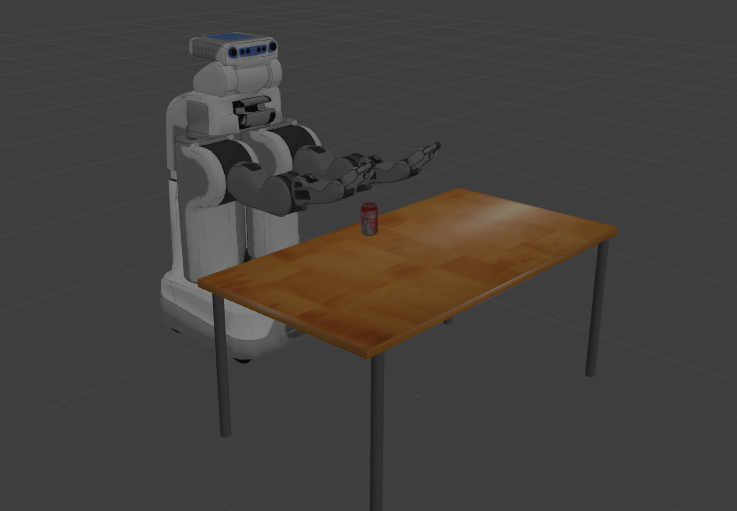
\includegraphics[height=8cm]{img/gazebo_pr2.png}
		\caption{An example simulation of the PR2 robot for testing object grasp operation}
		\label{fig:gazebo_pr2}
	\end{figure}

	\subsubsection{ROS and ros\_control integration}
	To integrate Gazebo with ROS ecosystem, a set of ROS packages named \textsf{gazebo\_ros\_pkgs} was created. They allow to start Gazebo as a ROS node that provides its functionality through ROS messages, services and parameters. They also contain various plugins for integrating sensors and a script for spawning a URDF model.

	\textsf{gazebo\_ros\_control} package was created, in order to integrate Gazebo with \textsf{ros\_control} framework. It consists of the following elements:
	\begin{itemize}
		\item \val{RobotHWSim} -- a base class for writing a hardware abstraction layer for a simulated robot model,
		\item \val{DefaultRobotHWSim} -- a generic implementation of the RobotHWSim interface. It reads transmission tags from URDF to link actuators to joints,
		\item \textbf{\textsf{gazebo\_ros\_control} plugin} -- a plugin for Gazebo simulator that implements control loop for ros\_control. It uses Controller Manager and RobotHWSim. To use it, the user can add the following lines to the URDF file:
		\lstinputlisting[language=XML]{lst/gazebo_ros_control.lst}
		\textsf{robotSimType} specifies the RobotHWSim implementation to use in the control loop. The \mbox{DefaultRobotHWSim} is sufficient in most cases, but the user can write their own implementation.
	\end{itemize}

	\begin{figure}[ht]
		\centering
		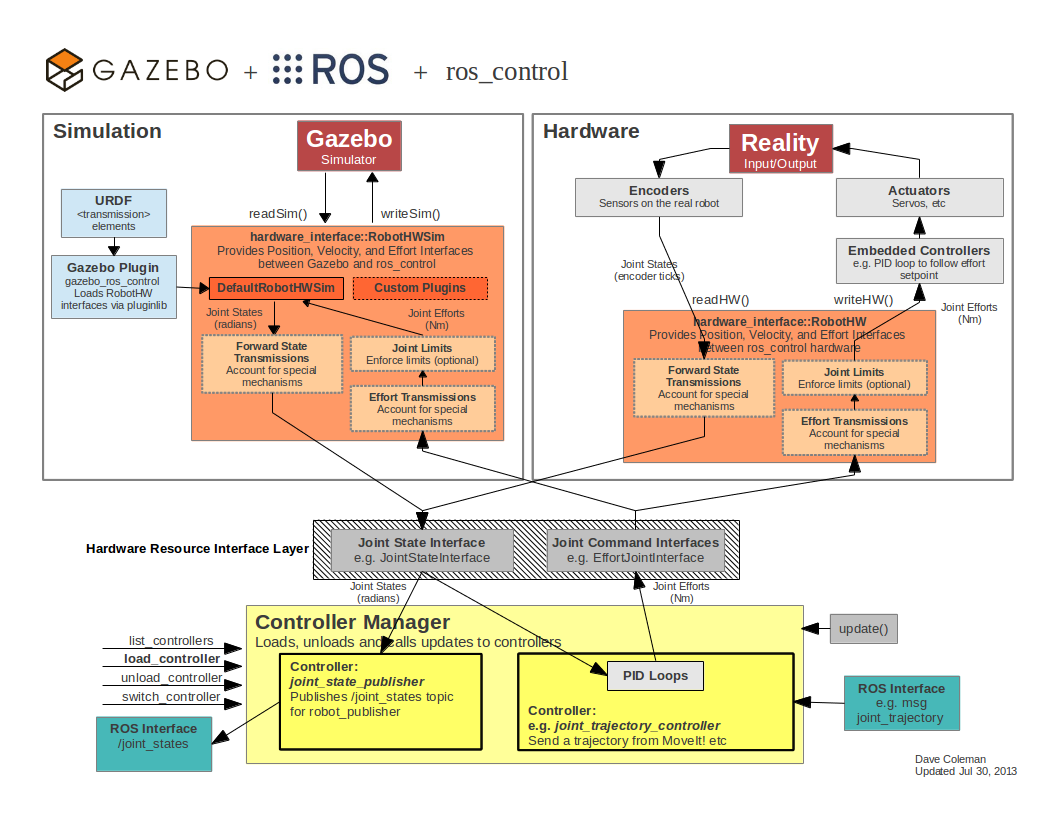
\includegraphics[width=\textwidth]{img/gazebo_control.png}
		\caption{Gazebo with ros\_control overview (Source: \cite{gazebo:ros_control})}
		\label{fig:gazebo_control}
	\end{figure}

\pagebreak

	\subsection{RUBI}
	Rover Universal Board Interface (RUBI) is a framework for easy, rapid and reliable integration of STM32 microcontroller-based devices with ROS. It was conceived by Cezary Siwek (former member of the \textit{Continuum} team) during works on \oldrovername as a way to quickly integrate sensor modules. It is continued to be used on the \rovername robot as a communication protocol for custom motor drivers.

	It consists of the following elements:
	\begin{itemize}
		\item \val{rubi\_server} -- a ROS node that keeps track of connected devices (referred to in RUBI as \textit{boards}) and exposes their capabilities to ROS topics. It communicates with the boards using a custom protocol over CAN (Common Area Network) bus. 
		% It utilizes CAN (Common Area Network) interfaces by using custom-designed protocol to communicate with the boards.
		\item \val{rubi\_client} -- a client library that implements the RUBI protocol. The current version of the library supports STM32 F-series microcontrollers and Linux.
		\item \val{rubi\_generic\_gui} -- an RQt plugin that provides a dynamically generated user interface for connected RUBI boards.

	\end{itemize}

	The usage of the framework is fairly simple. The client uses RUBI-specific macros to define fields which can either be read-only (server $\rightarrow$ client), write-only (server $\leftarrow$ client) or read-write (server $\leftrightarrow$ client). The fields are then accessible in the code as variables in the static memory of a program.

	\lstinputlisting[language=rubiC]{lst/rubi_client.lst}

	When the server connects to the board, it spawns topics that allow to access the fields. For this example, the following topics would be created:

	\lstinputlisting{lst/rubi_server.lst}

	Whenever a value on the board is changed, a new message is published on a corresponding \textsf{fields\_from\_board} topic. Publishing on a \textsf{fields\_to\_board} topic changes the value of the associated variable on the board. \textsf{reboot}, \textsf{sleep} and \textsf{wake} topics provide additional functionality for managing the board state.

	The result of using RUBI on \rovername rover is the ability to quickly integrate hot-pluggable physical devices with the ROS ecosystem without changing any of the code running on the robot's computer.


\chapter{Documentation of the ROS package stack}

This chapter dives deeper into the ROS packages that are the subject of this thesis. It describes the content of each package, provided ROS nodes, launch files, scripts, configuration files, etc.

It is worth noticing that the software for the \rovername robot is constantly evolving. The following documentation refers to the version of the software that has been frozen for the purposes of the thesis and parts of it may be not up-to-date in the near future.

\section{Overview of provided packages} \label{overview}

	The base ROS package stack for controlling and simulating the \rovername robot includes the following packages:

	\begin{itemize}
		\item \val{aleph2\_description} -- 
		contains the model of the \rovername robot in URDF format,
		\item \val{aleph2\_hardware\_interface} -- 
		provides a hardware abstraction layer implementation for \textsf{ros\_control} framework and a control loop node,
		\item \val{aleph2\_bringup} -- 
		contains configuration, launch files and additional scripts for starting \rovername base functionality,
		\item \val{aleph2\_gazebo} -- 
		contains configuration and launch files for simulating the \rovername robot in Gazebo.
	\end{itemize}

	The packages that are also required but not available in the ROS distribution and are not the subject of this thesis include:

	\begin{itemize}
		\item \val{kacanopen} -- provides a set of libraries for communication with devices that implement the CANopen protocol \cite{kacanopen2016}. The package was adapted by the \textit{Continuum} team to follow a file structure that is more consistent with the ROS ecosystem. 
		\item \val{nanotec\_driver} -- contains a C++ library that utilizes \textsf{kacanopen} to provide an interface for communication with \textit{Nanotec} motor drivers which are used extensively on the \rovername robot.
		\item \val{rubi\_server} -- contains the server node for communication with RUBI-enabled devices and message definitions for the ROS side of the protocol,
		\item \val{power\_msgs} -- contains the \textsf{PowerStatus} message definition that is used by the \textsf{power\_monitor} node.
	\end{itemize}

% \pagebreak

\section{aleph2\_description}

	The purpose of this package is to provide a URDF model of the \rovername robot that describes its visual, kinematic and physical properties. It uses \href{http://wiki.ros.org/xacro}{\textsf{xacro}} to make the description more human-readable, by using macros, math expressions, conditional blocks and by splitting the description into multiple files. 

	The package contents can be summarized by the following structure:

	\begin{figure}[H]
	\dirtree{%
		.1 aleph2\_description/.
			.2 meshes/
			\filedesc{3D models of robot parts in STL or COLLADA formats}.
			.2 textures/
			\filedesc{texture files used in RViz visualization}.
			.2 launch/
			\filedesc{launch files}.
			.2 urdf/.
				.3 aleph2.urdf.xacro
				\filedesc{main xacro file}.
				.3 aleph2.gazebo.xacro
				\filedesc{additional link and joint properties for simulation purposes in Gazebo}.
				.3 *.xacro
				\filedesc{other xacro files that are included by the main xacro file}.
				.3 aleph2.urdf
				\filedesc{An output urdf file generated from the main xacro file}.
			.2 rviz/ 
			\filedesc{display configuration files for RViz}.
			% .2 CMakeLists.txt.
			% .2 package.xml.
	}
	\end{figure}

	\subsection{Naming conventions}

		To make sure the names across the model are consistent, a set of naming conventions for links and joints has been established:
		\begin{itemize} 
			\item root link of the robot should be named \textsf{base\_link},
			\item link names should end with a \textsf{\_link} keyword if the link has any visual; collision or physical properties,
			\item if the link does not contain any properties and is only used as a reference frame, its name should contain a \textsf{\_frame} suffix,
			\item joint names should start with the name of the joint's child link (without the suffix) and end with a \textsf{\_joint} keyword,
			\item if the joint mimics other joint (contains \textsf{mimic} tag), its name should end with \textsf{\_mimic\_joint} suffix.
		\end{itemize}

		Fig. \ref{fig:aleph2_description} shows the graph representation of the \rovername URDF model that follows to the established naming conventions.

	\subsection{Launch files}
	
		\begin{itemize}
			\item \val{rviz.launch}\\
			Starts an RViz instance with a specified display configuration (see Fig. \ref{fig:description_rviz})

			\textbf{Arguments}:
			\begin{itemize}[itemsep=0pt, parsep=2pt, topsep=0pt]
				\item \textsf{rvizconfig} (\textsf{string}, default: \textsf{aleph2\_description/rviz/aleph2.rviz})\\
				path to the RViz display configuration file. The default configuration shows the robot model with the root link as the fixed reference frame.
			\end{itemize}

			\item \val{display.launch}\\
			Launches the 3D visualization of the \rovername robot in RViz with simulated joint states. It loads the \textsf{robot\_description} parameter to the Parameter Server, starts \textsf{robot\_state\_publisher} and \textsf{joint\_states\_publisher} nodes and includes \textsf{rviz.launch} file with default arguments.

			\textbf{Arguments}:
			\begin{itemize}[itemsep=0pt, parsep=2pt, topsep=0pt]
				\item \textsf{gui} (\textsf{bool}, default: \textsf{true})\\
				If set to \textsf{true}, \textsf{joint\_state\_publisher} will spawn a gui that allows adjusting joint positions with sliders.
				\item \textsf{model} (\textsf{string}, default: \textsf{aleph2\_description/urdf/aleph2.urdf.xacro})\\
				path to the URDF model in xacro format
			\end{itemize}
		\end{itemize}

	\begin{figure}[ht]
		\centering
		\captionsetup{margin=2cm}
		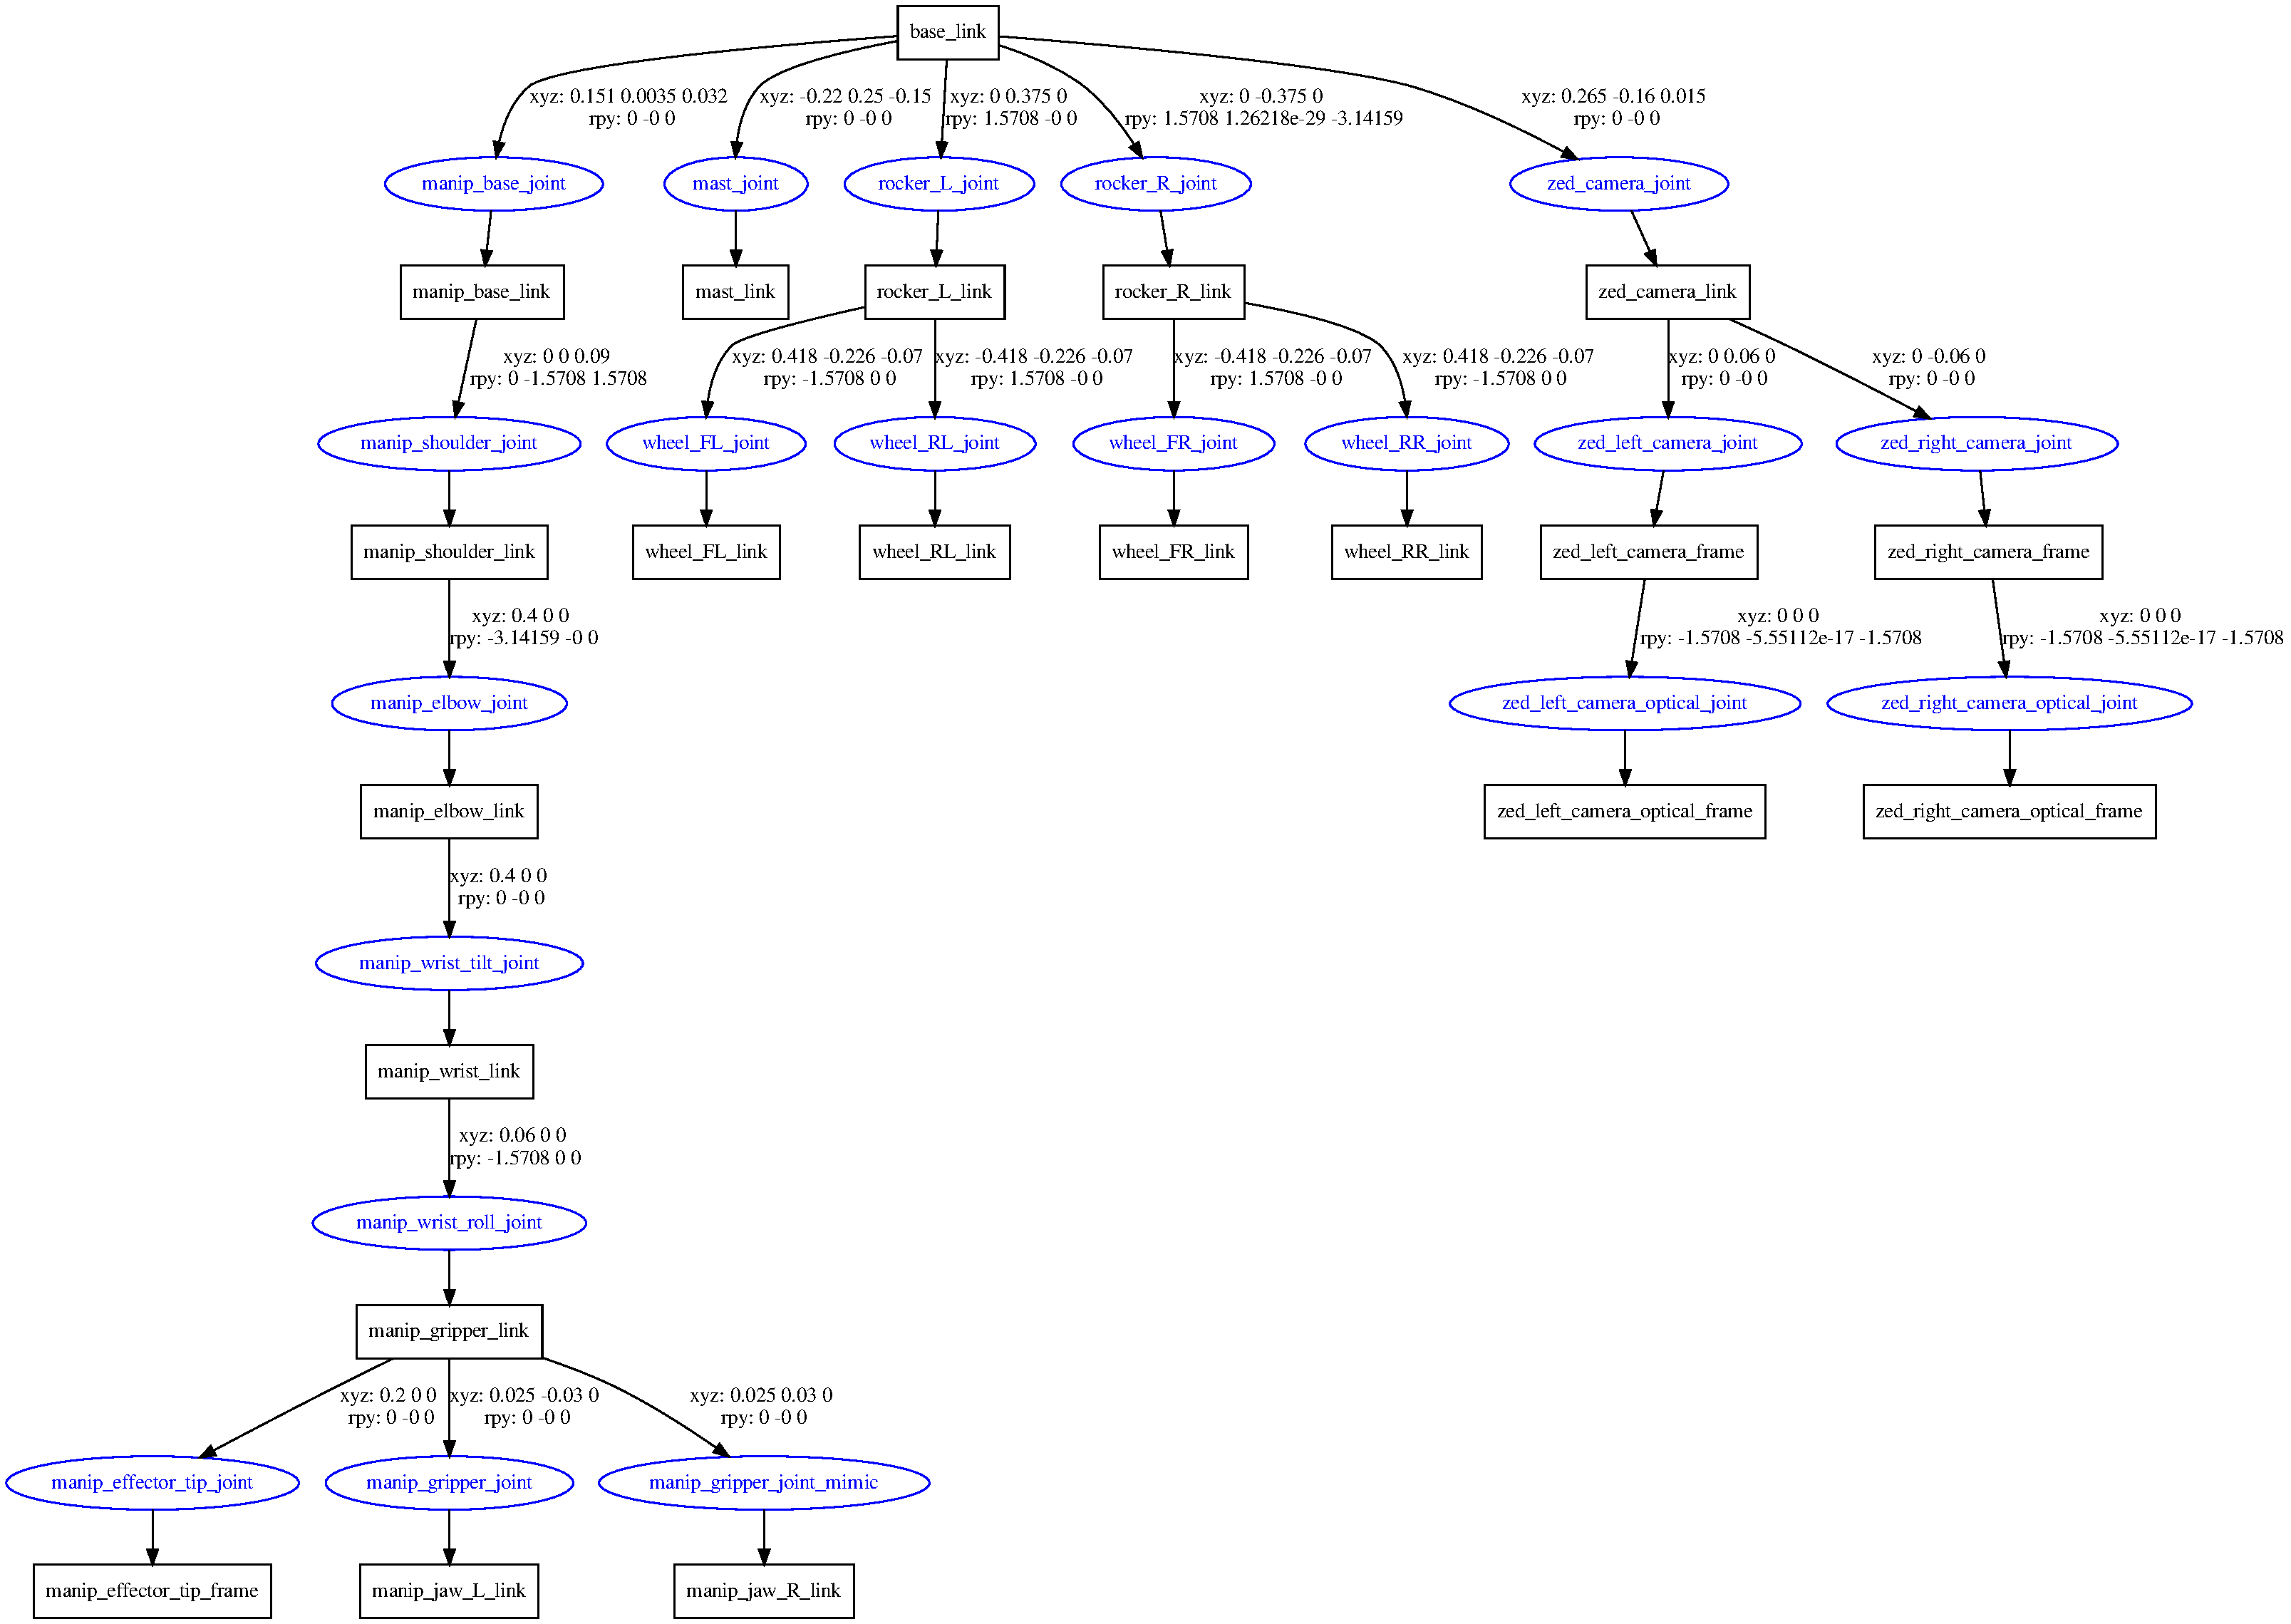
\includegraphics[width=\textwidth]{img/aleph2_description.pdf}
		\caption{A graph visualization of the URDF model generated from the \textsf{aleph2.urdf} file}
		\label{fig:aleph2_description}
	\end{figure}

	\begin{figure}[H]
		\centering
		\captionsetup{margin=2cm}
		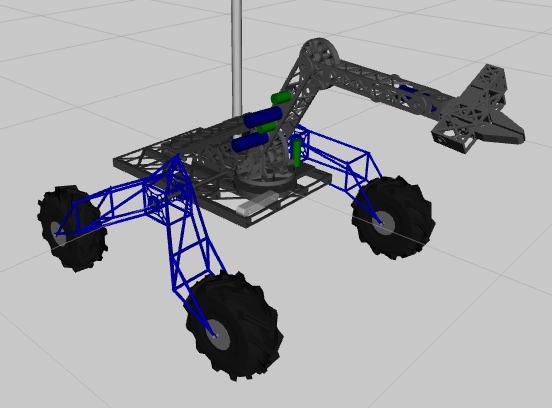
\includegraphics[width=\textwidth]{img/description_rviz.png}
		\caption{Visualization of the \rovername robot in RViz}
		\label{fig:description_rviz}
	\end{figure}

% \pagebreak

\section{aleph2\_hardware\_interface}
The package was created to provide an abstraction layer over the hardware running on \rovername that can be used with \textsf{ros\_control} framework. Although the abstraction was created for the needs of the aforementioned robot, its implementation is fully robot-agnostic and can be used with any configuration of the supported hardware.

\subsection{Libraries}
	\begin{itemize}
		\item \val{aleph2\_joint}\\
		Provides a set of classes that allow exposing capabilities of hardware controlling the joints of a robot via a common interface.

		\begin{figure}[ht]
			\centering
			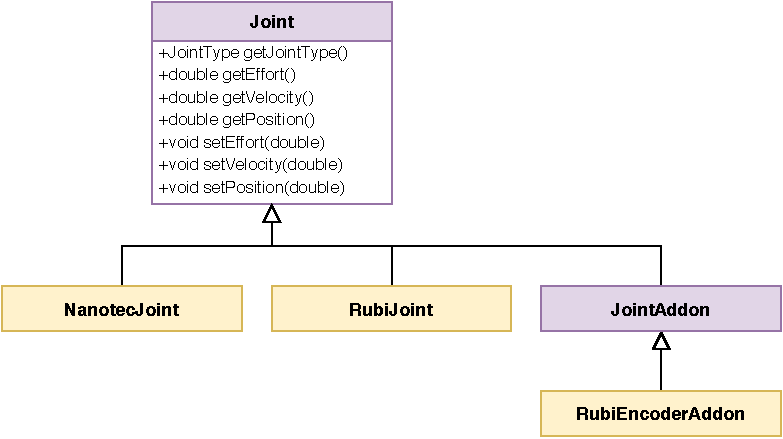
\includegraphics[width=\textwidth]{img/aleph2_joint.pdf}
			\caption{class hierarchy diagram for the \textsf{aleph2\_joint library}}
			\label{fig:aleph2_joint}
		\end{figure}

		\begin{description}[style=nextline]
			\item [Joint] A base class that provides a common interface for exposing capabilities of various joint types.
			\item [NanotecJoint] A derived class that exposes capabilities of a joint controlled by a \textit{Nanotec} motor driver. Apart from implementing the \textsf{Joint} interface, it provides dynamically reconfigurable parameters (see \cite{dynamic_reconfigute:wiki}) that allow setting motor's power and passive brakes.
			\item [RubiJoint] A derived class that exposes capabilities of a joint controlled by a RUBI-enabled board. It can implement any subset of the \textsf{Joint} interface by specifying only selected RUBI fields. If \textsf{home} field is specified, it creates a service which enables homing functionality for a joint.
			\item [JointAddon] A base class for extending or modifying joint's capabilities. It uses a decorator design pattern to overwrite the behavior of certain functions from \textsf{Joint} interface.
			\item [RubiEncoderAddon] A derived class that represents a RUBI-enabled position sensor. It overwrites the \textsf{getPosition()} method of a \textsf{Joint} instance.
		\end{description}

		\item \val{aleph2\_hw}\\
		Provides the \textsf{Aleph2HW} class which implements \textsf{RobotHW} interface for \textsf{ros\_control} framework. Upon initialization, it reads the hardware configuration from the Parameter Server, creates corresponding \textsf{Joint} instances, creates state and command handles for the joints and registers hardware interfaces.

		A sample configuration which explains the joint specification read by the \textsf{Aleph2HW} class can be found in the \textsf{config/template.yaml} file.

	\end{itemize}

\subsection{Nodes}

	\begin{itemize}
		\item \val{control\_loop}\\
		Initializes \textsf{Aleph2HW} instance, creates Controller Manager and starts a control loop for the \textsf{ros\_control} framework. In each loop cycle, it reads the data from the hardware, updates all active controllers and writes commands to the hardware.

		\textbf{Published topics}:
		\begin{itemize}[itemsep=0pt, parsep=2pt, topsep=0pt]
			\item \textsf{$\sim$usage} (type: \textsf{std\_msgs/Float32})\\
			the percentage of the expected cycle time used. Calculated and published at the end of each cycle.
		\end{itemize}

		\textbf{Parameters}:
		\begin{itemize}[itemsep=0pt, parsep=2pt, topsep=0pt]
			\item \textsf{$\sim$loop\_rate} (\textsf{int}, default: \textsf{20})\\
			frequency (in Hz) at which the control loop is operating.
			\item \textsf{$\sim$spinner\_threads} (\textsf{int}, default: \textsf{4})\\
			the number of threads used to asynchronously process callbacks from ROS subscribers
			\item \textsf{$\sim$hw\_namespace} (\textsf{string})\\
			If set, Aleph2HW and Controller Manager will use a relative namespace for ROS node handles.
		\end{itemize}

		The node will also spawn additional topics and services used by the Controller Manager, loaded controllers and \textsf{Aleph2HW} joints.
	\end{itemize}

\section{aleph2\_bringup}
The purpose of this package is to provide a configuration that enables starting the base functionality of the \rovername rover. It contains configuration files in YAML format, ROS launch files and additional scripts (single-file nodes) that are applicable only to the real robot.

	\subsection{Configuration files}

	\begin{figure}[H] % prevent splitting across pages
	\dirtree{%
		.1 config/.
			.2 control/
			\filedesc{Configuration files for the control software}.
				.3 drivetrain/.
					.4 joints.yaml
					\filedesc{joints specification, read by the \textsf{Aleph2HW} instance}.
					.4 joint\_limits.yaml
					\filedesc{joint limits specification, read by the \textsf{Aleph2HW} instance}.
					.4 controllers.yaml
					\filedesc{a set of controllers with their parameters to load to the Controller Manager}.
				.3 manip/.
				.3 gimbal/.
			.2 rosbags.yaml
			\filedesc{rosbag descriptions for the \textsf{rosbag\_recorder} node}.
	}
	\end{figure}


	The configuration for the \rovername control software has been split into 3 subsystems:

	\begin{itemize}
		\item \val{drivetrain}\\
		The \textsf{drivetrain} subsystem is responsible for robot's capability to navigate through terrain. It consists of 4 wheels controlled by \textit{Nanotec} motor drivers and uses differential drive kinematics for teleoperation.

		\textbf{Joints}:
		\begin{itemize}[itemsep=0pt, parsep=2pt, topsep=0pt]
			\item \textsf{wheel\_FL\_joint} (type: \textsf{nanotec})
			\item \textsf{wheel\_FR\_joint} (type: \textsf{nanotec})
			\item \textsf{wheel\_RL\_joint} (type: \textsf{nanotec})
			\item \textsf{wheel\_RR\_joint} (type: \textsf{nanotec})
		\end{itemize}

		\textbf{Controllers}:
		\begin{itemize}[itemsep=0pt, parsep=2pt, topsep=0pt]
			\item \textsf{joint\_state\_controller/JointStateController}
			\item \textsf{velocity\_controllers/JointVelocityController} -- one for each joint
			\item \textsf{diff\_drive\_controller/DiffDriveController} 
		\end{itemize}

		\item \val{manip}\\
		A 5 degrees of freedom robotic arm attached to the \rovername rover. It uses  RUBI-enabled motor drivers to control the actuators.

		\textbf{Joints}:
		\begin{itemize}[itemsep=0pt, parsep=2pt, topsep=0pt]
			\item \textsf{manip\_base\_joint} (type: \textsf{rubi})
			\item \textsf{manip\_shoulder\_joint} (type: \textsf{rubi})
			\item \textsf{manip\_elbow\_joint} (type: \textsf{rubi})
			\item \textsf{manip\_wrist\_tilt\_joint} (type: \textsf{rubi})
			\item \textsf{manip\_wrist\_roll\_joint} (type: \textsf{rubi})
			\item \textsf{manip\_gripper\_joint} (type: \textsf{rubi})
		\end{itemize}

		\textbf{Controllers}:
		\begin{itemize}[itemsep=0pt, parsep=2pt, topsep=0pt]
			\item \textsf{joint\_state\_controller/JointStateController}
			\item \textsf{effort\_controllers/JointEffortController} -- one for each joint
			\item \textsf{effort\_controllers/JointVelocityController} -- one for each joint 
			\item \textsf{effort\_controllers/JointPositionController} -- one for each joint
			\item \textsf{effort\_controllers/JointTrajectoryController}
		\end{itemize}

		\item \val{gimbal}\\
		The \textsf{gimbal} subsystem consists of 4 pan--tilt--zoom--focus cameras that are controlled by RUBI-enabled boards. 

		\textbf{Joints}:
		\begin{itemize}[itemsep=0pt, parsep=2pt, topsep=0pt]
			\item \textsf{gimbalN\_pan} (type: \textsf{rubi})
			\item \textsf{gimbalN\_tilt} (type: \textsf{rubi})
			\item \textsf{gimbalN\_zoom} (type: \textsf{rubi})
			\item \textsf{gimbalN\_focus} (type: \textsf{rubi})
		\end{itemize}
		where $N \in \{0,1,2,3\}$

		\textbf{Controllers}:
		\begin{itemize}[itemsep=0pt, parsep=2pt, topsep=0pt]
			\item \textsf{joint\_state\_controller/JointStateController}
			\item \textsf{velocity\_controllers/JointVelocityController} -- one for each joint
		\end{itemize}
	\end{itemize}

	The \textsf{rosbags.yaml} file contains definitions of the following rosbags:
	\begin{itemize}[itemsep=0pt, parsep=2pt, topsep=0pt]
		\item \textsf{control} -- data from the controllers, node logs, state of the robot
		\item \textsf{sensors} -- sensor data, such as IMU, GNSS readings, odometry measurements, occupancy maps
		\item \textsf{cameras} -- camera images, depth maps, point cloud data
	\end{itemize}

	\subsection{Nodes}
		\begin{itemize}
			\item \val{power\_monitor}\\
			Periodically reads voltage and current from INA3221 monitors located at the Jetson TX2 board and publishes the measurements on a ROS topic.

			\textbf{Published topics}:
			\begin{itemize}[itemsep=0pt, parsep=2pt, topsep=0pt]
				\item \textsf{power\_status} (type: \textsf{power\_msgs/PowerStatus})\\
				cumulative reading from all INA monitors
			\end{itemize}

			\textbf{Parameters}:
			\begin{itemize}[itemsep=0pt, parsep=2pt, topsep=0pt]
				\item \textsf{$\sim$update\_rate} (\textsf{int}, default: \textsf{2})\\
				frequency in Hz with which the readings are published
			\end{itemize}

			\item \val{rosbag\_recorder}\\
			Records rosbags specified in private parameters and dumps all parameters in the Parameter Server to a YAML file.

			\textbf{Parameters}:
			\begin{itemize}[itemsep=0pt, parsep=2pt, topsep=0pt]
				\item \textsf{$\sim$rosbags/\{name\}} (\textsf{string list})\\
				list of topic names for rosbag \{name\}
				\item \textsf{$\sim$active} (\textsf{string list})\\
				names of rosbags to record
				\item \textsf{$\sim$log\_folder} (\textsf{string}, default: \textsf{/var/log/ros/rosbags})\\
				path of the directory where the files are stored. Parameters are dumped into \textsf{log\_folder/\{date\}/parameters.yaml} and each rosbag is recorded into \textsf{log\_folder/\{date\}/\{name\}.bag}
			\end{itemize}
		\end{itemize}

	\subsection{Launch files}

		\begin{itemize}
			\item \val{drivetrain\_control.launch}\\
			Loads the drivetrain configuration to the Parameter Server, starts a control loop for the drivetrain subsystem, and loads the controllers to the Controller Manager. Starts \textsf{JointStateController} and \textsf{DiffDriveController}.

			\textbf{Arguments}:
			\begin{itemize}[itemsep=0pt, parsep=2pt, topsep=0pt]
				\item \textsf{output} (\textsf{string}, default: \textsf{screen})\\
				controls where the standard output of each started node is sent. Must be either \textsf{screen} or \textsf{log}.
				\item \textsf{loop\_rate} (\textsf{int}, default: \textsf{20})\\
				the rate in Hz at which the control loop is operating.
			\end{itemize}

			\item \val{manip\_control.launch}\\
			Loads the manip configuration to the Parameter Server, starts a control loop for the manip subsystem, and loads the controllers to the Controller Manager. Starts \textsf{JointStateController} and \textsf{JointEffortController} for each joint.

			\textbf{Arguments}:
			\begin{itemize}[itemsep=0pt, parsep=2pt, topsep=0pt]
				\item \textsf{output} (\textsf{string}, default: \textsf{screen})
				\item \textsf{loop\_rate} (\textsf{int}, default: \textsf{30})
			\end{itemize}

			\item \val{gimbal\_control.launch}\\
			Loads the gimbal configuration to the Parameter Server, starts a control loop for the gimbal subsystem, and loads the controllers to the Controller Manager. Starts \textsf{JointStateController} and \textsf{JointVelocityController} for each joint.

			\textbf{Arguments}:
			\begin{itemize}[itemsep=0pt, parsep=2pt, topsep=0pt]
				\item \textsf{output} (\textsf{string}, default: \textsf{screen})
				\item \textsf{loop\_rate} (\textsf{int}, default: \textsf{10})
			\end{itemize}

			\item \val{rosbags.launch}\\
			Starts the \textsf{rosbag\_recorder} node with the configuration stored in the YAML file.

			\textbf{Arguments}:
			\begin{itemize}[itemsep=0pt, parsep=2pt, topsep=0pt]
				\item \textsf{record\_cameras} (\textsf{bool}, default: \textsf{false})\\
				by default, only \textsf{control} and \textsf{sensors} rosbags are started, if this parameter is set to \textsf{true}, the \textsf{cameras} rosbag is also started. 
			\end{itemize}

			\item \val{aleph2\_bringup.launch}\\
			Starts the base functionality of the \rovername robot. It includes all the previous launch files and also loads the URDF model to the Parameter Server and starts \textsf{robot\_state\_publisher}, \textsf{rubi\_server} and \textsf{power\_monitor} nodes.

			\textbf{Arguments}:
			\begin{itemize}[itemsep=0pt, parsep=2pt, topsep=0pt]
				\item \textsf{output} (\textsf{string}, default: \textsf{log})
				\item \textsf{model} (\textsf{string}, default: \textsf{aleph2\_description/urdf/aleph2.urdf.xacro})\\
				path to the URDF model in xacro format
			\end{itemize}


		\end{itemize}

\section{aleph2\_gazebo}
This package was created to provide Gazebo-related functionality for the \rovername robot. It contains controllers configuration, sample world description and launch files that enable starting the simulated environment for the robot.

\subsection{Configuration files}

	\begin{itemize}
		\item \val{pid\_gains.yaml}\\
		the tuning of the PID controllers that are used by \textsf{gazebo\_ros\_control} plugin to simulate velocity-controlled joints.
		\item \val{controllers.yaml}\\
		description of a set of controllers to be loaded by the Controller Manager. It combines \textsf{drivetrain} and \textsf{manip} subsystems described in the  \textsf{aleph2\_bringup} package except that they have a common \textsf{JointStateController} and the PID tuning is different.
		\item \val{aleph2.world}\\
		description of a sample, empty world in SDF format.
	\end{itemize}

\subsection{Launch files}

	\begin{itemize}
		\item \val{world.launch}\\
		Starts Gazebo simulator with a specified world description.

		\textbf{Arguments}:
		\begin{itemize}[itemsep=0pt, parsep=2pt, topsep=0pt]
			\item \textsf{output} (\textsf{string}, default: \textsf{screen})\\
			controls where the standard output of each started node is sent. Must be either \textsf{screen} or \textsf{log}.
			\item \textsf{world} (\textsf{string}, default: \textsf{aleph2\_gazebo/worlds/aleph2.world})\\
			path to the world description in SDF format.
			\item \textsf{gui} (\textsf{bool}, default: \textsf{true})\\
			whether to start Gazebo with a graphical interface.
			\item \textsf{paused} (\textsf{bool}, default: \textsf{false})\\
			if set to \textsf{true}, simulation will be paused at start.
			\item \textsf{use\_sim\_time} (\textsf{bool}, default: \textsf{true})\\
			controls the value of \textsf{use\_sim\_time} parameter set at the Parameter Server.
			\item \textsf{debug} (\textsf{bool}, default: \textsf{false})\\
			if set to \textsf{true}, Gazebo will be started inside the GDB debugger.
		\end{itemize}

		\item \val{spawn\_model.launch}\\
		Loads the URDF model to the Parameter Server and spawns the robot in a simulated world. The default model launches the \textsf{gazebo\_ros\_control} plugin with \textsf{DefaultRobotHWSim} implementation.

		\textbf{Arguments}:
		\begin{itemize}[itemsep=0pt, parsep=2pt, topsep=0pt]
			\item \textsf{output} (\textsf{string}, default: \textsf{screen})
			\item \textsf{model} (\textsf{string}, default: \textsf{aleph2\_description/urdf/aleph2.urdf.xacro})\\
			path to the URDF model in xacro format
			\item \textsf{fixed} (\textsf{bool}, default: \textsf{false})\\
			if set to \textsf{true}, the robot's root link will be fixed to the world frame.
		\end{itemize}

		\item \val{spawn\_controllers.launch}\\
		Loads the controller configuration to the Parameter Server, loads all the controllers to the Controller Manager, starts \textsf{JointStateController}, \textsf{DiffDriveController} for \textsf{drivetrain} subsystem and \textsf{JointEffortController} for each joint in \textsf{manip} subsystem. Also starts \textsf{robot\_state\_publisher}.

		\textbf{Arguments}:
		\begin{itemize}[itemsep=0pt, parsep=2pt, topsep=0pt]
			\item \textsf{output} (\textsf{string}, default: \textsf{screen})
		\end{itemize}

		\item \val{aleph2\_gazebo.launch}\\
		Starts the base functionality of the \rovername robot in a simulated environment. It includes all the previously described launch files in this package.

		\textbf{Arguments}:
		\begin{itemize}[itemsep=0pt, parsep=2pt, topsep=0pt]
			\item \textsf{output} (\textsf{string}, default: \textsf{log})
			\item \textsf{world} (\textsf{string}, default: \textsf{aleph2\_gazebo/worlds/aleph2.world})\\
			path to the world description in SDF format.
			\item \textsf{gui} (\textsf{bool}, default: \textsf{true})\\
			whether to start Gazebo with a graphical interface.
		\end{itemize}

	\end{itemize}

	\begin{figure}[ht]
		\centering
		\captionsetup{margin=2cm}
		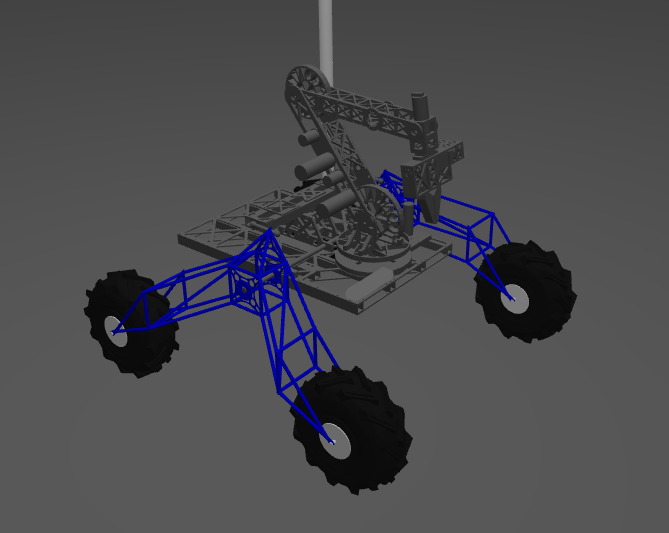
\includegraphics[width=0.85\textwidth]{img/gazebo.png}
		\caption{\rovername model spawned in Gazebo simulated world}
		\label{fig:gazebo}
	\end{figure}

\chapter{Usage instructions}
The software was designed to be used with \textsf{NVIDIA Jetson TX2} board which is the main computer on the \rovername rover. It can, however, work with basically any system that supports ROS. This chapter contains instructions on how to install the software and use its functionalities described in the documentation. 

The steps were tested on \textsf{Ubuntu 18.04} system which is the main platform supported by the latest ROS distribution (at the time this thesis was written). The process of installation may be slightly different for other distributions.

The instructions may use some terminology related to catkin workspaces that is explained in \cite{usage:workspace}.

{ % stop paragraph indentation
\setlength{\parindent}{0pt}

\section{Prerequisites}
Before the packages can be built, the following dependencies need to be installed on the system:

\begin{itemize}
	\item \val{ROS Melodic} -- at least the \textsf{ros\_base} package stack, see the official ROS Wiki page \cite{usage:ros_installation} for installation instructions,
	\item \val{rosdep} -- a command-line tool for installing system dependencies \cite{usage:rosdep}. Available in ROS repository as \textsf{python-rosdep} package.
	\item \val{catkin-tools} -- a package that provides command line tools for working with ROS buildsystem \cite{usage:catkin}. Available in ROS repository as \textsf{python-catkin-tools} package.
\end{itemize}

You will also need to initialize \textsf{rosdep} sources:
\begin{lstlisting}[language=mybash]
sudo rosdep init
\end{lstlisting}

% \pagebreak

\section{Building}

\begin{enumerate}

\item Start by creating the directories for the catkin workspace and the source space:
\lstinputlisting[language=mybash, firstline=1, lastline=2]{lst/installation.lst}

\item (Optionally) Set the workspace to explicitly extend the \textsf{melodic} result space:
\lstinputlisting[language=mybash, firstline=5, lastline=5]{lst/installation.lst}

\item Put the packages you want to build in the source space. For launching the simulation, only \textsf{aleph2\_description} and \textsf{aleph2\_gazebo} are required. If you want to build the whole package stack, you will need to download addition packages mentioned in \ref{overview}:
\lstinputlisting[language=mybash, firstline=7, lastline=11]{lst/installation.lst}

\item Update \textsf{apt} and \textsf{rosdep} package information:
\lstinputlisting[language=mybash, firstline=13, lastline=14]{lst/installation.lst}

\item Use \textsf{rosdep} to install system dependencies:
\lstinputlisting[language=mybash, firstline=16, lastline=17]{lst/installation.lst}

\item (Optionally) Specify the install directory if you want to use the install space:
\lstinputlisting[language=mybash, firstline=19, lastline=19]{lst/installation.lst}

\item Build the packages:
\lstinputlisting[language=mybash, firstline=21, lastline=21]{lst/installation.lst}

\item Source the environmental setup file from the result space:
\lstinputlisting[language=mybash, firstline=23, lastline=23]{lst/installation.lst}
If you used the install space:
\lstinputlisting[language=mybash, firstline=24, lastline=24]{lst/installation.lst}

\item (Optionally) Add the above line to \textsf{.bashrc} file to source the result space automatically at the start of every terminal session:
\lstinputlisting[language=mybash, firstline=26, lastline=26]{lst/installation.lst}

\end{enumerate}

\section{Launching}
The first thing one can do to test whether the packages were built correctly and are working is to run the RViz visualization with a simulated robot state:
\lstinputlisting[language=mybash, firstline=1, lastline=1]{lst/launching.lst}
This will launch a basic ROS infrastructure for robot state publishing, RViz with the robot visualization and a GUI that allows changing the current joint positions. Close RViz or type \textsf{Ctrl+C} to exit.

The next thing you can do is to test the simulation environment.\\
Start by launching an empty world in Gazebo simulator:
\lstinputlisting[language=mybash, firstline=3, lastline=3]{lst/launching.lst}

then, spawn the \rovername robot model into the world by opening another terminal session and typing: 
\lstinputlisting[language=mybash, firstline=4, lastline=4]{lst/launching.lst}

and load the controllers to the Controller Manager by typing:
\lstinputlisting[language=mybash, firstline=5, lastline=5]{lst/launching.lst}

You can also use the \textsf{aleph2\_gazebo.launch} file which includes the three previous launch files instead of running each one separately:
\lstinputlisting[language=mybash, firstline=7, lastline=7]{lst/launching.lst}
Add \textsf{gui:=false} if you want to run the Gazebo simulator headless.

To visualize the current robot state (seen by the simulated hardware) in RViz, type:
\lstinputlisting[language=mybash, firstline=9, lastline=9]{lst/launching.lst}

The simulated robot should now be ready for operation.\\
To command the \textsf{DiffDriveController}, you need to publish on the \textsf{cmd\_vel} topic. You can send messages using the \textsf{rostopic} tool, like this:
\lstinputlisting[language=mybash, firstline=11, lastline=11]{lst/launching.lst}
This should command the robot to drive with the linear speed of 1 meter per second and the angular speed of 1 radian per second.

By default, only the effort controllers are started for the \textsf{manip} subsystem. These controllers can set the torque applied to a joint. For example, to set the torque of 100 Nm (in the reverse direction) on the \textsf{shoulder} joint, you would write:
\lstinputlisting[language=mybash, firstline=13, lastline=13]{lst/launching.lst}

To send position commands to the arm joint, you need to stop the effort controller and start the position controller first (they cannot be running at the same time). To do this, you need to make a call to the \textsf{switch\_controller} service, for example by using the \textsf{rosservice} tool: 
\lstinputlisting[language=mybash, firstline=15, lastline=15]{lst/launching.lst}
or by using \textsf{rqt\_controller\_manager} which offers a graphical interface for managing the running controllers.

Now, you should be able to set the position on the \textsf{shoulder} joint:
\lstinputlisting[language=mybash, firstline=17, lastline=17]{lst/launching.lst}

To run the same functionality on the real robot (and a little more), you can use the \textsf{aleph2\_bringup.launch} file:
\lstinputlisting[language=mybash, firstline=19, lastline=19]{lst/launching.lst}

The ROS API for the real and simulated rover is nearly identical except that on the real robot each subsystem creates a separate Controller Manager instance in its own namespace.\\
The corresponding \textsf{switch\_controller} call on the real robot would look like this:
\lstinputlisting[language=mybash, firstline=21, lastline=21]{lst/launching.lst}

} % paragraph indentation

\chapter{Conclusion}
It is fair to say that the new control software for the \rovername rover meets the goals described in section \ref{goals}. It is a powerful tool for integrating new hardware (as well as software) and provides a great base for students to further develop the rover. 

\section{Ways to improve the software}
The software is very useful as it is but some parts of it can be improved and certain functionalities can be added. The following problems (with their solutions) have been identified: 

\begin{itemize}
	\item The \textsf{Joint} instances created by \textsf{Aleph2HW} expose additional functionalities to the ROS ecosystem. This breaks a little the concept of \textsf{ros\_control} framework that assumes the capabilities of a robot are exposed only by the hardware interfaces and can be accessed only by the controllers loaded by the Controller Manager. A proper solution would be to create appropriate hardware interfaces and implement them in \textsf{Aleph2HW} and then load controllers that would expose these additional capabilities to ROS topics, services or parameters.  
	\item The \textsf{gazebo\_ros\_control} spawns one Controller Manager instance for all subsystems of the robot, but the configuration for the real robot assumes one control loop for each subsystem and thus multiple Controller Manager instances in different namespaces. This results in the ROS API between the real and simulated robot not being fully-compatible. An easy solution that addresses this issue has not been found yet.
	\item \textit{Nanotec} motor drivers can be operated in several modes that include Torque (effort), Velocity or Position. Despite that, the \textsf{Aleph2HW} class starts every \textsf{Nanotec} joint in Velocity mode and registers handles only for the velocity interface. The best fix for this issue would be to add a \textsf{mode} parameter to the \textsf{Nanotec} joint specification that sets the operation mode and registered hardware interface.
	\item The hardware abstraction supports changing the operation mode of a joint at runtime but it does not respect the fact that certain joint types may need an additional method call to change the operation mode. Adding a \textsf{setMode()} method to \textsf{Joint} interface and implementing it in derived classes may be a good solution.
	\item The \textsf{Aleph2HW} implementation does not differentiate between joints and actuators. It assumes there is a one-to-one mapping of joint position, effort etc. Perhaps a better solution would be to read only the actuator specification and use \textsf{ros\_control} transmissions, populated from URDF \textsf{transmission} tags, to link actuators to joints.
\end{itemize}

\section{Next steps}
There is a couple of steps to be taken, in order to prepare the robot for the competition challenges. The steps include:

\begin{itemize}
	\item \textbf{Integrating sensors} -- adding sensors, such as IMU or GNSS to the real robot; integrating the sensors with the URDF model and adding Gazebo plugins that simulate their behavior; making sure the ROS API between the real and simulated sensor is compatible,
	\item \textbf{Simulating challenge tasks} -- creating a simulation environments (worlds) for Gazebo that simulate the tasks the robot will have to accomplish on competition challenges.
	\item \textbf{Integrating the robotic arm with MoveIt} -- creating a configuration package for MoveIt Motion Planning Framework that would make use of the \textsf{\mbox{JointTrajectoryController}} running in the \textsf{manip} subsystem; creating an IKFast Kinematics Solver plugin for the arm,
	\item \textbf{Modeling the kinematic chain of the suspension} -- adding position sensors to the rover's suspension mechanism; modyfing the URDF model so that the exact state of the rockers and differential bar can be visualized by the sensor readings; simulating the rocker suspension in Gazebo by modeling a closed-loop kinematic chain.
\end{itemize}

\bibliographystyle{unsrt}
\bibliography{bibliography}

\end{document}
